\section{Diagrammi di Attività}{
	\subsection{Presentazione dei diagrammi}{
		In questa sezione sono presenti i diagrammi di attività di APIMarket. Essi rappresentano il flusso logico degli utenti che percorrono tutte le funzionalità dell'applicazione. Ogni diagramma sarà accompagnato da una breve descrizione.
	}
	\subsection{Attività principali}{
		\begin{figure}[ht]
			\centering
			\includegraphics[width=0.7\textwidth]{img/attivitaPrincipali}
			\caption{Diagrammi di attività - Attività principali}
			Questo diagramma rappresenta le operazioni principali che è possibile fare non appena aperta l'applicazione web. E' possibile autenticarsi, registrarsi o eseguire ricerche. 
		\end{figure}	
	}
	\subsection{Autenticazione utente} {
		\begin{figure}[ht]
			\centering
			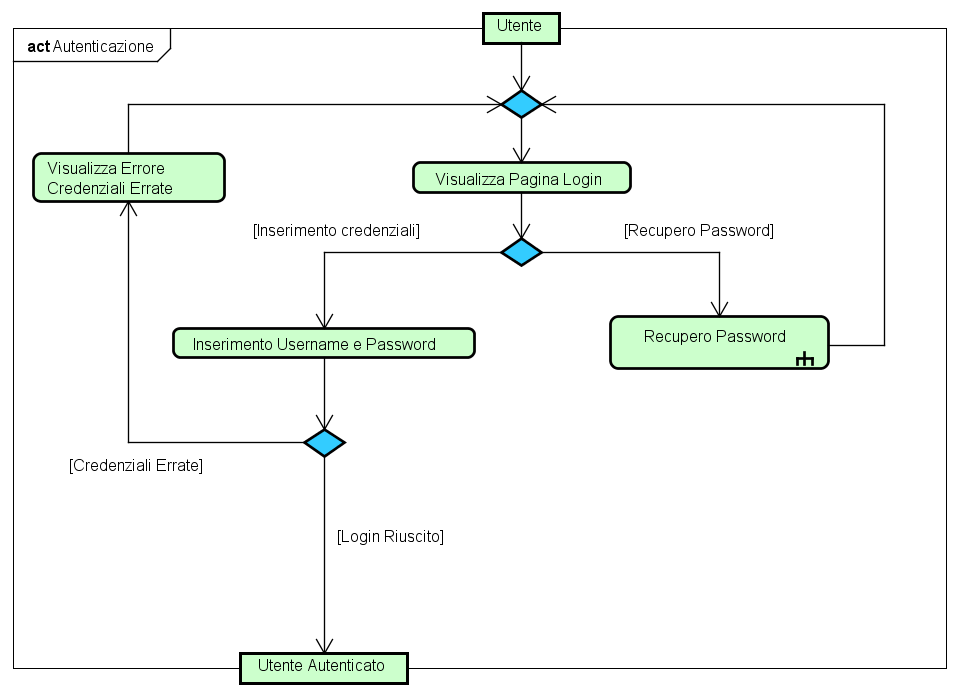
\includegraphics[width=0.7\textwidth]{img/autenticazioneUtente}
			\caption{Diagrammi di attività - Autenticazione utente}
			Questo diagramma rappresenta il meccanismo di autenticazione di un utente. Prima di tutto si accede alla pagina di login dove è possibile inserire i propri dati d'accesso. Se i dati sono corretti si procede al login, altrimenti si ritorna sulla pagina con un errore segnalato. E' anche possibile effettuare una procedura di recupero password. 
		\end{figure}
	}
	\subsection{Recupero password}{
		\begin{figure}[ht]
			\centering
			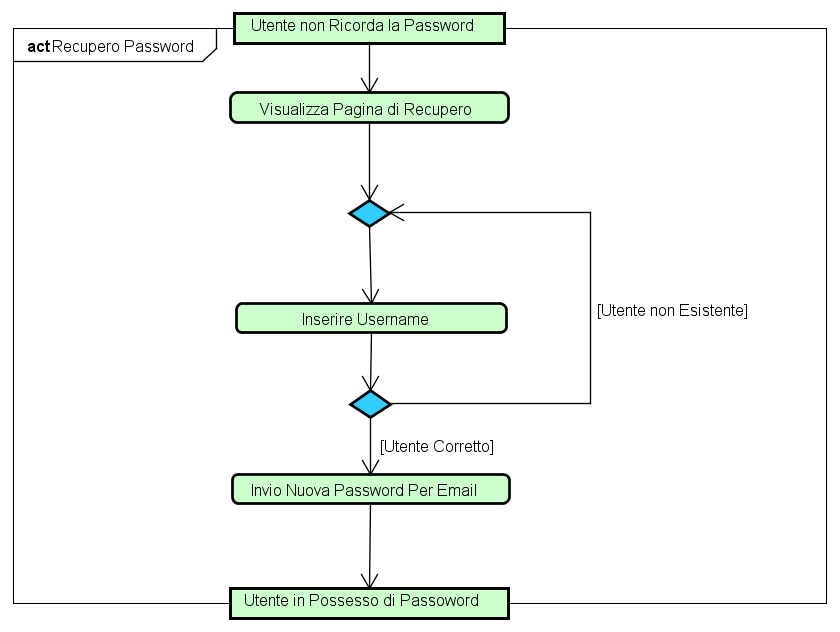
\includegraphics[width=0.7\textwidth]{img/recuperoPassword}
			\caption{Diagrammi di attività - Recupero password}
			Questo diagramma illustra la modalità di recupero password. Viene visualizzata una pagina in cui viene richiesto l'username. In seguito ad una conferma viene resettata la password e inviata per email.
		\end{figure}	
	}
	\subsection{Registrazione utente}{
		\begin{figure}[ht]
			\centering
			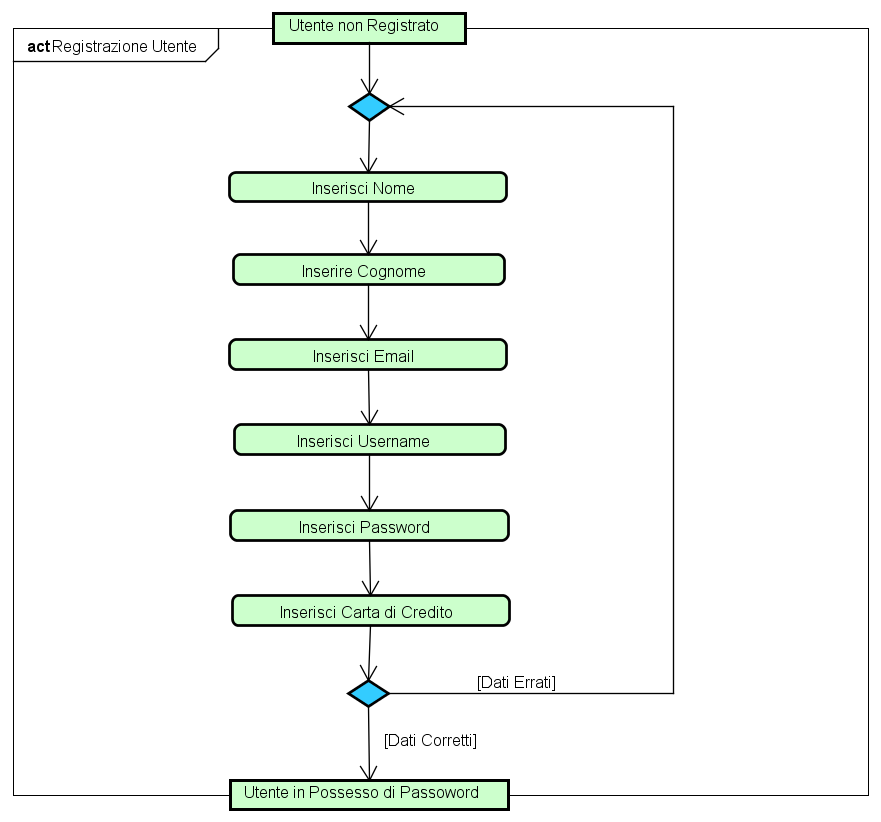
\includegraphics[width=0.7\textwidth]{img/registrazioneUtente}
			\caption{Diagrammi di attività - Registrazione utente}
			Questo diagramma rappresenta il meccanismo di registrazione di un nuovo utente. Vengono richieste in ordine nome, cognome, email, username, password, carta di credito. Se il sistema individua un errore lo segnala. Quando non ci sono più errori allora è possibile registrare il nuovo utente. 
		\end{figure}
	}
	\subsection{Accesso pagina utente}{
		\begin{figure}[ht]
			\centering
			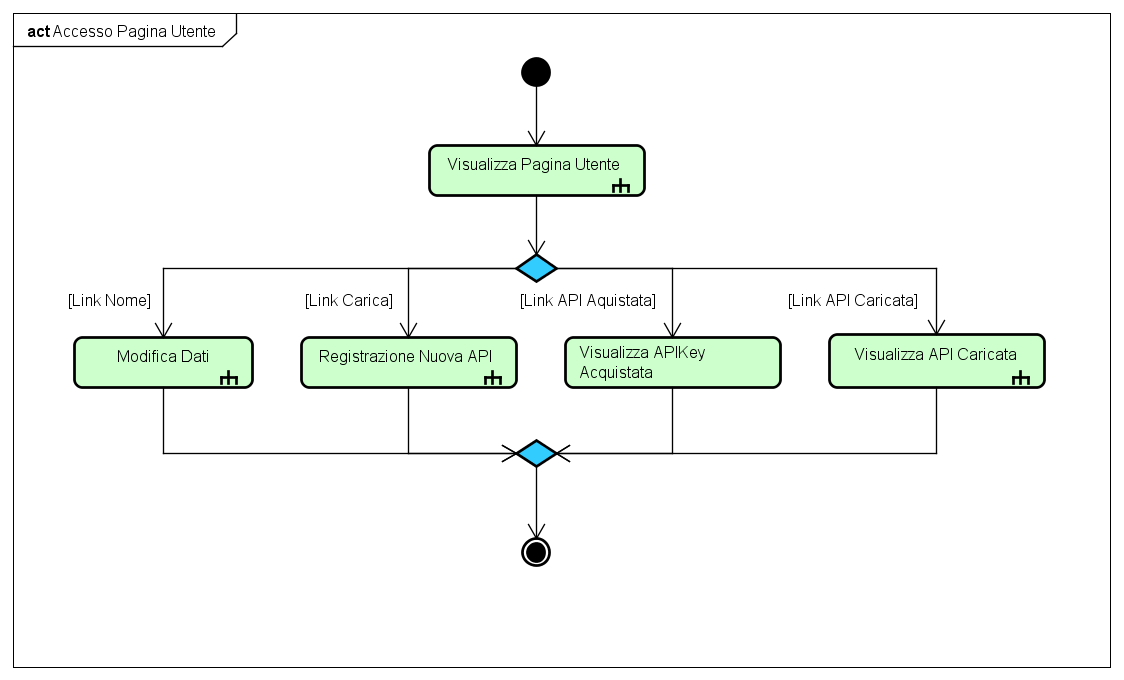
\includegraphics[width=0.7\textwidth]{img/accessoPaginaUtente}
			\caption{Diagrammi di attività - Accesso pagina utente}
			Questo diagramma rappresenta l'accesso da parte di un utente autenticato alla propria pagina utente. Una volta visualizzata la pagina è possibile modificare i propri dati personali, registrare una nuova API, visualizzare le APIKey acquistate o visualizzare le proprie API registrate. 
		\end{figure}
	}
	\subsection{Visualizza pagina utente}{
		\begin{figure}[ht]
			\centering
			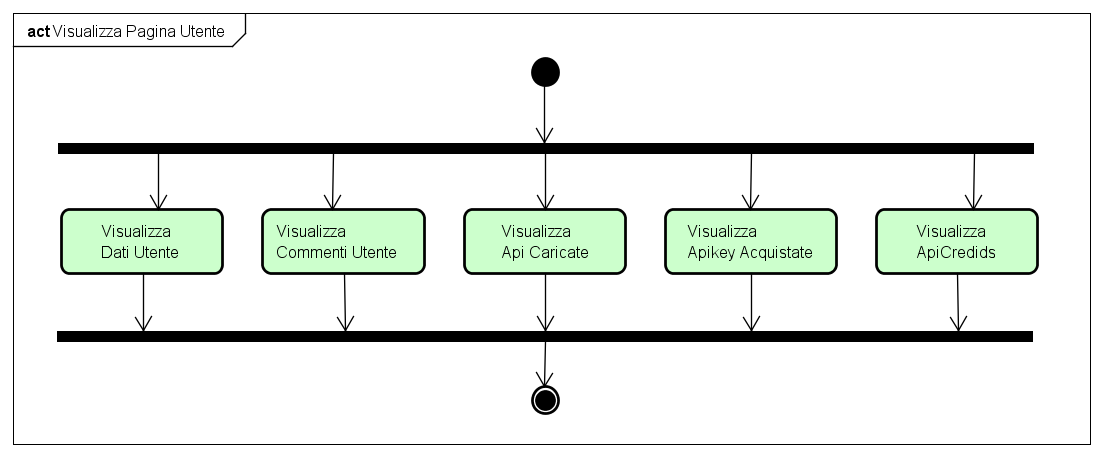
\includegraphics[width=0.7\textwidth]{img/visualizzaPaginaUtente}
			\caption{Diagrammi di attività - Visualizza pagina utente}
			Questo diagramma mostra ciò che viene visualizzato nella pagina utente.  
		\end{figure}	
	}	
	\subsection{Modifica dati}{
		\begin{figure}[ht]
			\centering
			\includegraphics[width=0.7\textwidth]{img/modificaDati}
			\caption{Diagrammi di attività - Modifica dati}
			Questo diagramma rappresenta il meccanismo per la modifica dei dati sul proprio profilo. Viene richiesto di modificare il dato scelto che verrà controllato, se è valido allora la modifica andrà a buon fine, altrimenti verrà segnalato un errore. 
		\end{figure}	
	}
	\subsection{Registrazione nuova API}{
		\begin{figure}[ht]
			\centering
			\includegraphics[width=0.7\textwidth]{img/registrazioneNuovaApi}
			\caption{Diagrammi di attività - Registrazione nuova API}
			Questo diagramma mostra il procedimento per la registrazione di una nuova API. 
		\end{figure}
	}
	\subsection{Visualizza API caricate}{
		\begin{figure}[ht]
			\centering
			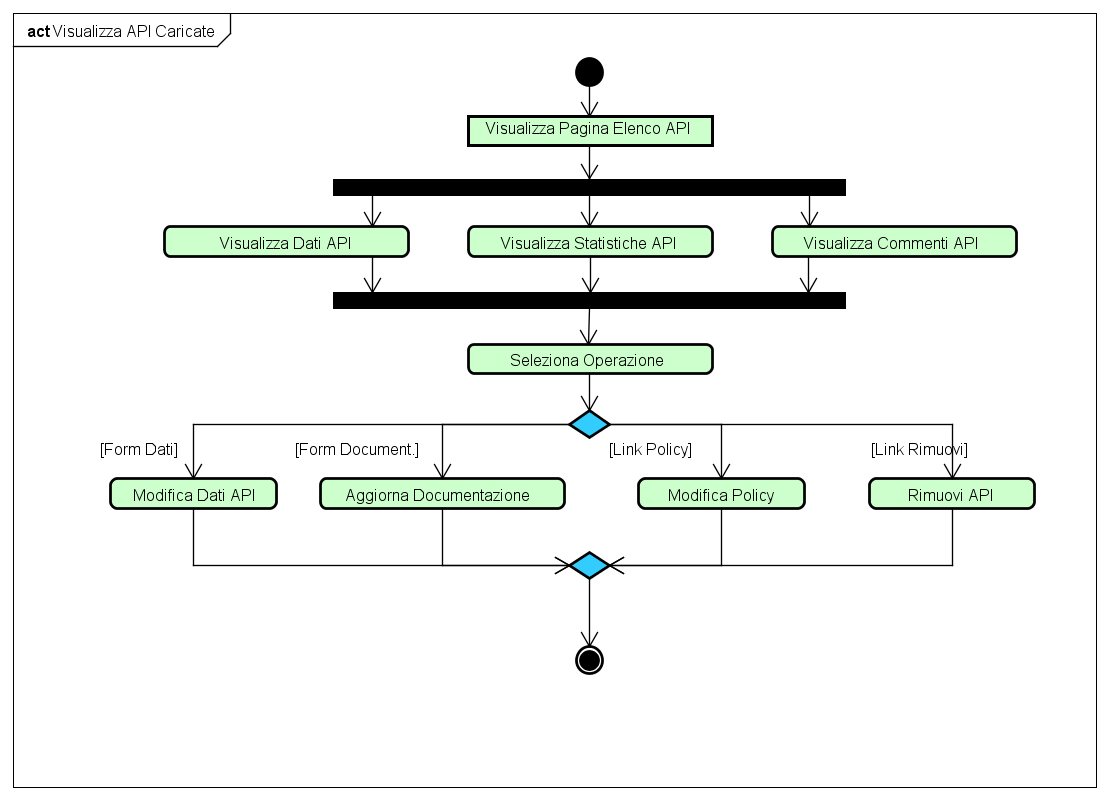
\includegraphics[width=0.7\textwidth]{img/visualizzaApiCaricate}
			\caption{Diagrammi di attività - Visualizza API caricate}
			Questo diagramma rappresenta la visualizzazione delle API registrate dall'utente. Una volta visualizzate tutte le informazioni utili è possibile modificare i dati dell'API, aggiornare la sua documentazione, modificare le policy di vendita o rimuovere l'API dal market. 
		\end{figure}	
	}
	\subsection{Ricerca}{
		\begin{figure}[ht]
			\centering
			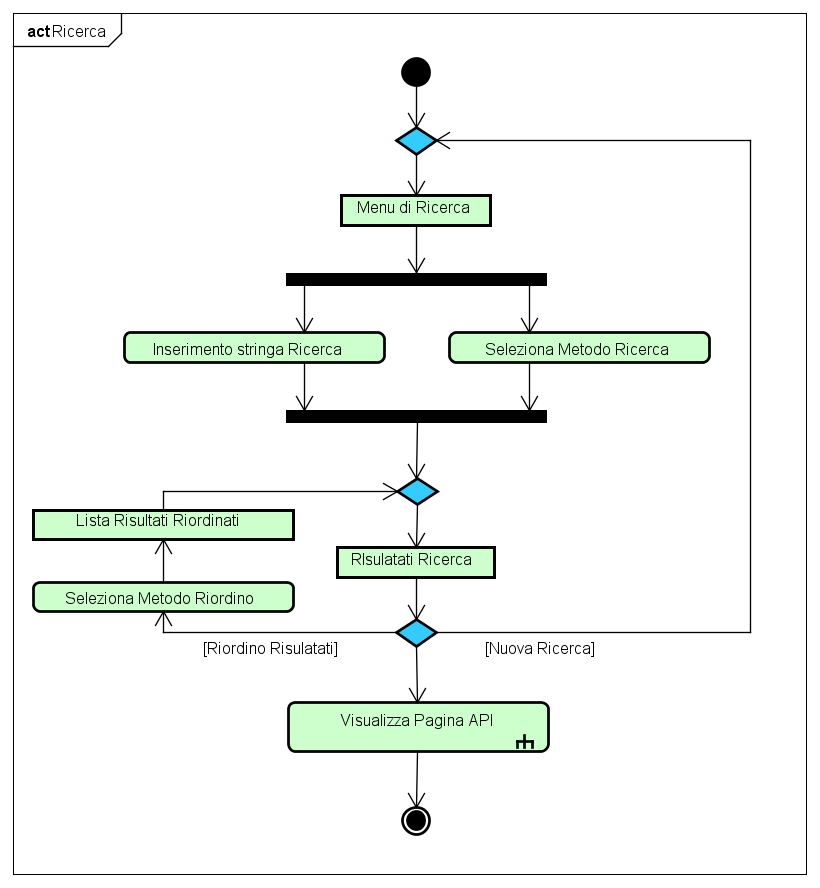
\includegraphics[width=0.7\textwidth]{img/ricerca}
			\caption{Diagrammi di attività - Ricerca}
			Questo diagramma mostra le modalità di ricerca su APIMarket. Una volta impostata la ricerca è possibile visualizzare i risultati della ricerca e riordinare i risultati. Infine è possibile osservare le pagine delle API ricercate. 
		\end{figure}	
	}
	\subsection{Visualizza pagina API}{
		\begin{figure}[ht]
			\centering
			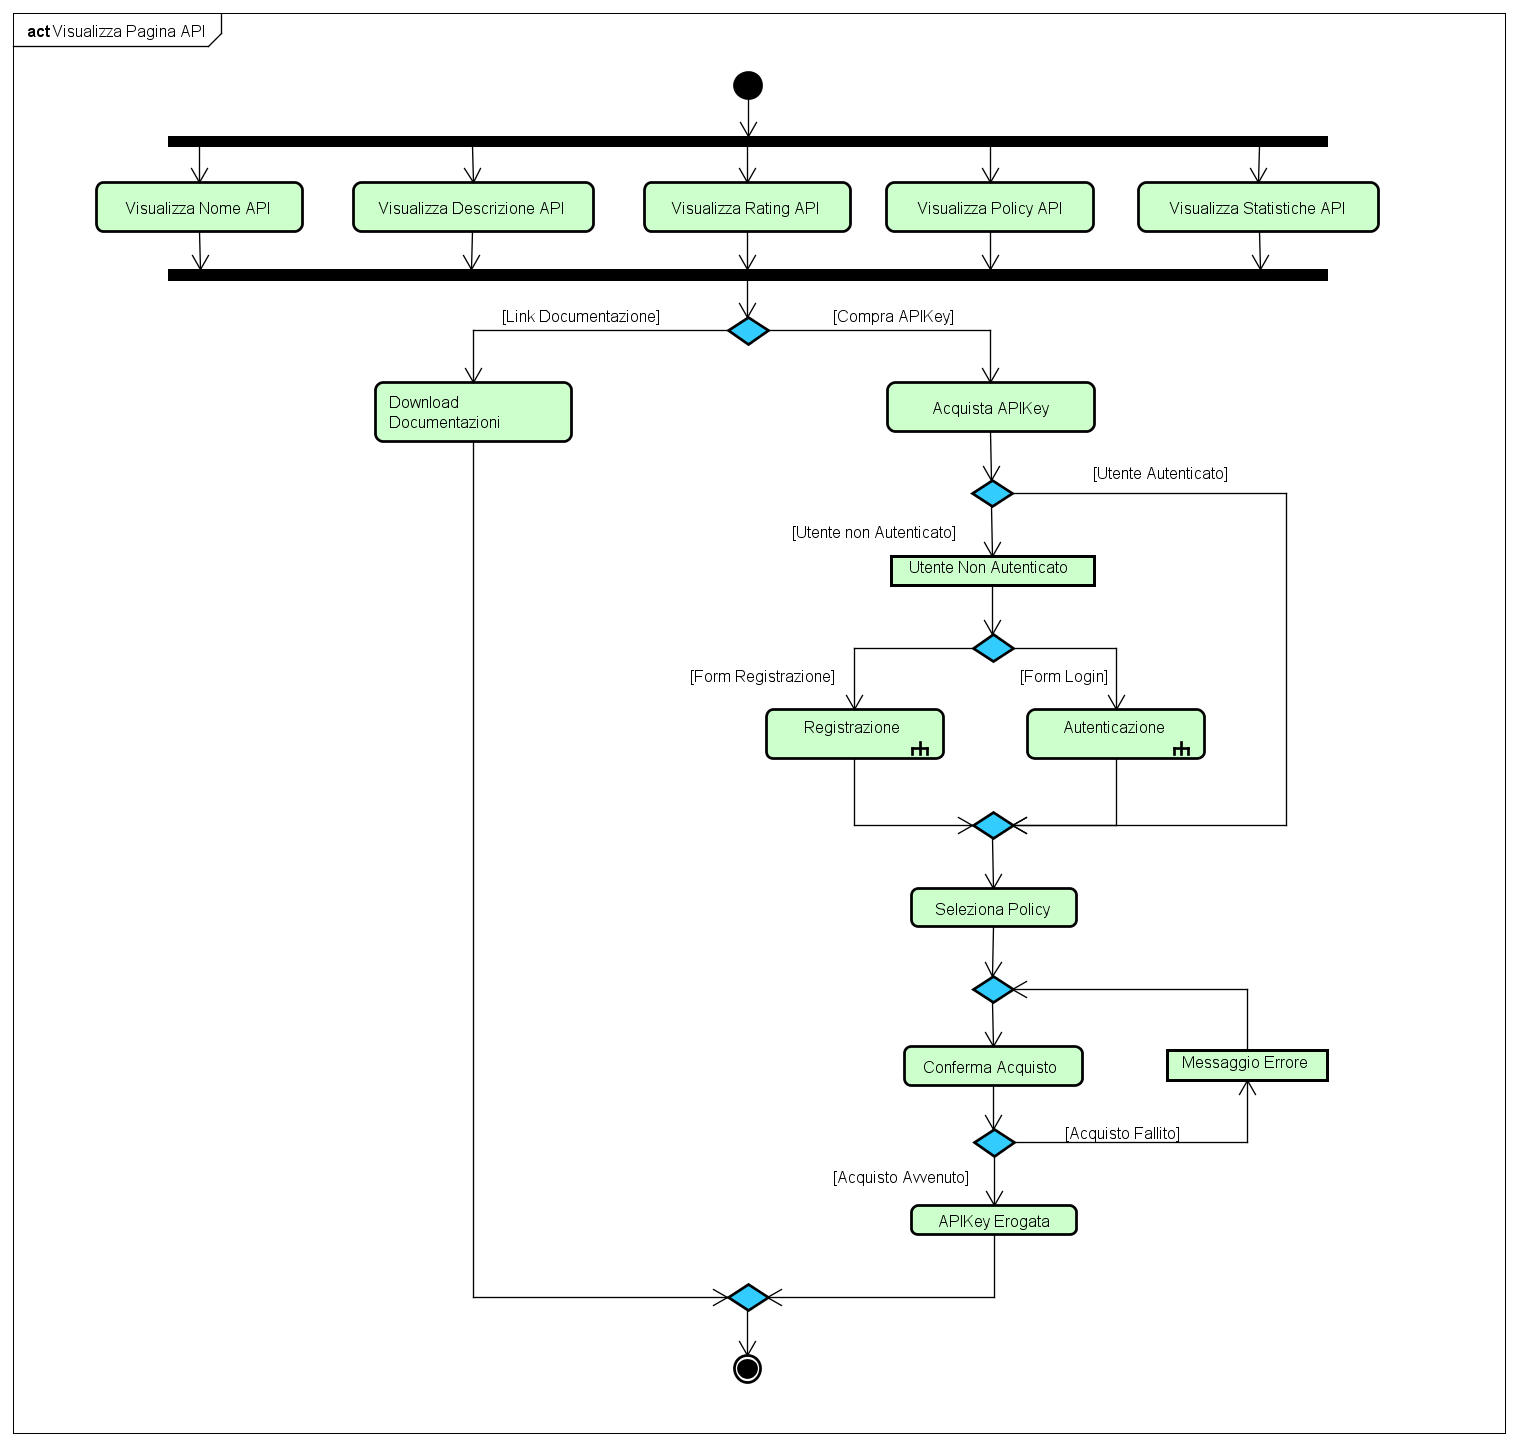
\includegraphics[width=0.7\textwidth]{img/visualizzaPaginaApi}
			\caption{Diagrammi di attività - Visualizza pagina API}
			Questo diagramma rappresenta la visualizzazione della pagina di vendita dell'API cercata. Una voltà visualizzati tutti dati relativi a quell'API l'utente può decidere di acquistare una APIKeyu o di scaricare la documentazione relativa. E' necessario essere autenticati per acquistare una APIKey e avere un sufficiente numero di APICredits.  
		\end{figure}	
	}
	\subsection{Utente amministrativo}{
		\begin{figure}[ht]
			\centering
			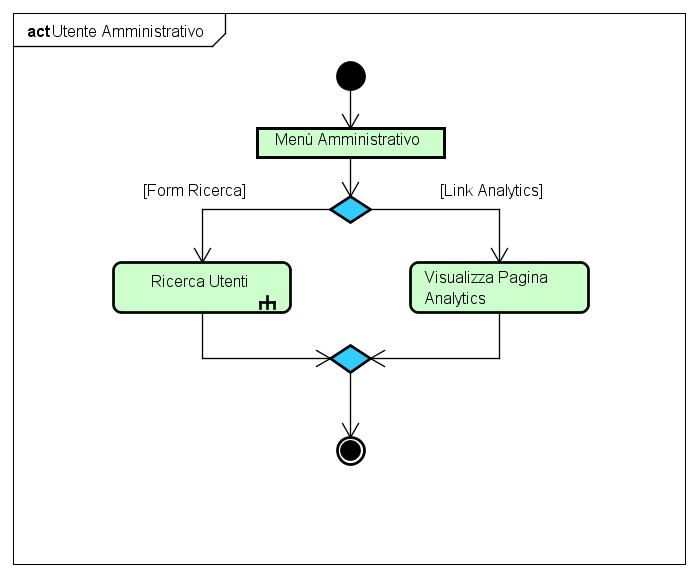
\includegraphics[width=0.7\textwidth]{img/utenteAmministrativo}
			\caption{Diagrammi di attività - Utente Amministrativo}
			Questo diagramma illustra le funzionalità dell'utente Amministrativo. Egli può ricercare utenti e visionare le statistiche del sito. Quando accede alle pagine di altri utenti può modificarle. 
		\end{figure}	
	}
}